\chapter{Schema Implementation}\label{implementation}
This chapter focuses on the implementation of the data models discussed in chapter \ref{design}. Each database management system has its own procedure for initiating a new collection, table, node or column family. This chapter discusses the methods and strategies I imposed to create the database solution designs; with a focus on any challenges faced in doing so.

\section{Creating database systems}\label{dbcreate}
Once the process of modelling of the database systems was complete, the next stage was to transform the model plan into actual databases. For each database system, this was relatively simple. However, this brought limitations and restrictions which I had to understand to fully achieve my target model.

\subsection{MySQL}
The MySQL data model consists of 8 tables; AnatomyStructures, Assays, Genes, Publications, Sources, Specimens, Stages and TextAnnotations. Each of which are discussed in detail in section \ref{mysqldesign}. The creation of these tables was a relatively straightforward undertaking. The ease in which I found this process may be due to my previous experience of using MySQL. The intuitive and logical way in which relational databases are constructed also makes implementing a data model, an all-round elementary procedure. An example of how a table is created in MySQL can be found in the code snippet \ref{code:mysqlass} below. This code illustrates the creation of the Assays table, the indexes and the constraints.
\newpage
\vspace*{\fill}
\begin{lstlisting}[language=SQL, caption=Creation of Assays table in MySQL., label=code:mysqlass]
--
-- Table structure for table `Assays`
--
CREATE TABLE IF NOT EXISTS `Assays` (
  `emage_id` int(11) NOT NULL,
  `type` varchar(255) DEFAULT NULL,
  `probe_id` varchar(255) DEFAULT NULL,
  `source_id` int(11) NOT NULL,
  `specimen_id` int(11) NOT NULL,
  `stage_id` int(11) NOT NULL,
) ENGINE=InnoDB DEFAULT CHARSET=utf8;
--
-- Indexes for table `Assays`
--
ALTER TABLE `Assays`
  ADD PRIMARY KEY (`emage_id`),
  ADD KEY `source_id` (`source_id`),
  ADD KEY `specimen_id` (`specimen_id`),
  ADD KEY `stage_id` (`stage_id`);
--
-- Constraints for table `Assays`
--
ALTER TABLE `Assays`
  ADD CONSTRAINT `fk_Assays_Sources` FOREIGN KEY (`source_id`)
  REFERENCES `Sources` (`source_id`),
  ADD CONSTRAINT `fk_Assays_Specimens` FOREIGN KEY (`specimen_id`)
  REFERENCES `Specimens` (`id`),
  ADD CONSTRAINT `fk_Assays_Stages` FOREIGN KEY (`stage_id`)
  REFERENCES `Stages` (`id`);
\end{lstlisting}
\vspace*{\fill}
\newpage

As shown in lines 4 - 11 of code snippet \ref{code:mysqlass}, the creation of each column takes the form of column name then data type with length and the value i.e. null or not null. The character set for each table by default, was set to utf8. It is noteworthy that the key values were not  instantiated at time of creation. This was as a result of an experiment aiming evaluate the effect index keys and constraints had at time of data load for each database. The full discussion and outcome of this experiment can be found in section \ref{loaddiscussion}.

MySQL tables are linked by joining the (unique) primary key of one column to the (unique or non unique) foreign key of another. Lines 15-19 in code snippet \ref{code:mysqlass} are where the key columns are create. Lines 23 - 29 are where the foreign key constraints are expressed. The notion of keys joining tables can often be confusing to understand on first encounter. Primary and foreign keys are, in most cases, confined to integer values. This is as a result of data containing inconsistent, ambiguous and non universal values. For example, a primary key may have the value ``Mouse'' and a foreign key may have the value ``mouse''. Both valid strings however as they do not match exactly the join would fail. The rigidity of these constructs have as many advantages as they do disadvantages. While the concept of joining two tables on matching integers seems logical, many situations occur where there is no unique ID present in the dataset. Therefore the ID has to be manually created based on the data available.

The process described was repeated for each of the tables in the devised data model. Creating multiple tables and joining them together in MySQL is relatively straightforward. While the formality of definitively expressing each term, and its data type, then stipulating the index keys and constraints, can be a tedious process. It is done so in a logical and objective manner which makes it coherent and understandable for the programmer.

\subsection{MongoDB}\label{mongocreate}
Creating a document inside a MongoDB collection (the equivalent to a MySQL table) is done by inserting field and value pairs. Each time a new field and value pair is inserted into a collection a new document is created. By default, each document in a collection is provided with a unique ID which has an object data type. ObjectIds are small, fast to generate, and ordered. These values consist of 12-bytes, where the first four bytes are a timestamp that reflect the ObjectId's creation \cite{md}. A unique ID can also be manually created for each document, if desired. For example, if a dataset has a unique identifier which will be used as a reference, this can be implemented by expressing the ``\_id'' field to a value. For example ``\_id : 1234'' would by the ID of a single document. This concept is illustrated in line 2 of code snippet \ref{code:mongoinsert}.

MongoDB is an extremely flexible data store. It accepts multiple different data types; from the standard string, double and boolean values to the more complex regular expressions and even Javascript code. By default, any value without a type specified will be presumed to be either a string or integer value. This attribute is common of NoSQL systems. It adds to the simplicity and smooth process of implementing a data model.

Documents can be created by either manually inserting on the command line, or by conducting a data dump. The latter is discussed in more detail in section \ref{mongoload}. Code snippet \ref{code:mongoinsert} below is an example of how a document can be created and data inserted from the command line.

Creating documents in MongoDB is an extremely simple process. It is unlikely that one would manually insert a large volume of data using the previously discussed \textit{db.collection.insert(\{\})} method. However, it is more likely that one would use this insertion process for adding additional data to an already implemented database, as opposed to creating from scratch. For example the EMAGE dataset contains around 200,000 entries. Inserting the full dataset using this methodology, while valid, would certainly not be the optimal solution. An explanation defining the full procedure into how I created the MongoDB documents can be found in section \ref{mongoload}.

An important design decision, which has to be taken prior to model implementation, is whether to create multiple collections or embed data within a document. A comprehensive evaluation of the advantages and disadvantages of this is discussed in section \ref{mongodesign}. The key difference; between the two approaches, are that within a multiple collection database, one is required to write multiple queries and also undertake client side application level processing. This is for the same outcome as writing a single line query using an embedded structure. All embedded data is available in a single document and can be accessed by a single query. The decision to choose between the two modelling designs should be based purely on a case by case basis. Separate collections are recommended if you need to select individual documents and would like more control over querying \cite{md}. Conversley embedded documents are recommended when you want the entire document all at once \cite{md}.

As discussed in section \ref{mongodesign} and illustrated in code snippet \ref{code:mongoinsert}, the MongoDB data model I have designed uses the embedded document approach. A good way of thinking of the embedded data concept is as document in a document. For example, in hierarchical terms, a document can have many fields, some with child fields as opposed to absolute values. Figure \ref{fig:embedded} illustrates an example of a document which has 3 fields and 3 values, one of which is an embedded document. The field named ``publication'' has 2 embedded (child) values which provide more information in the same collection about the same document.\begin{figure}[H]\begin{center}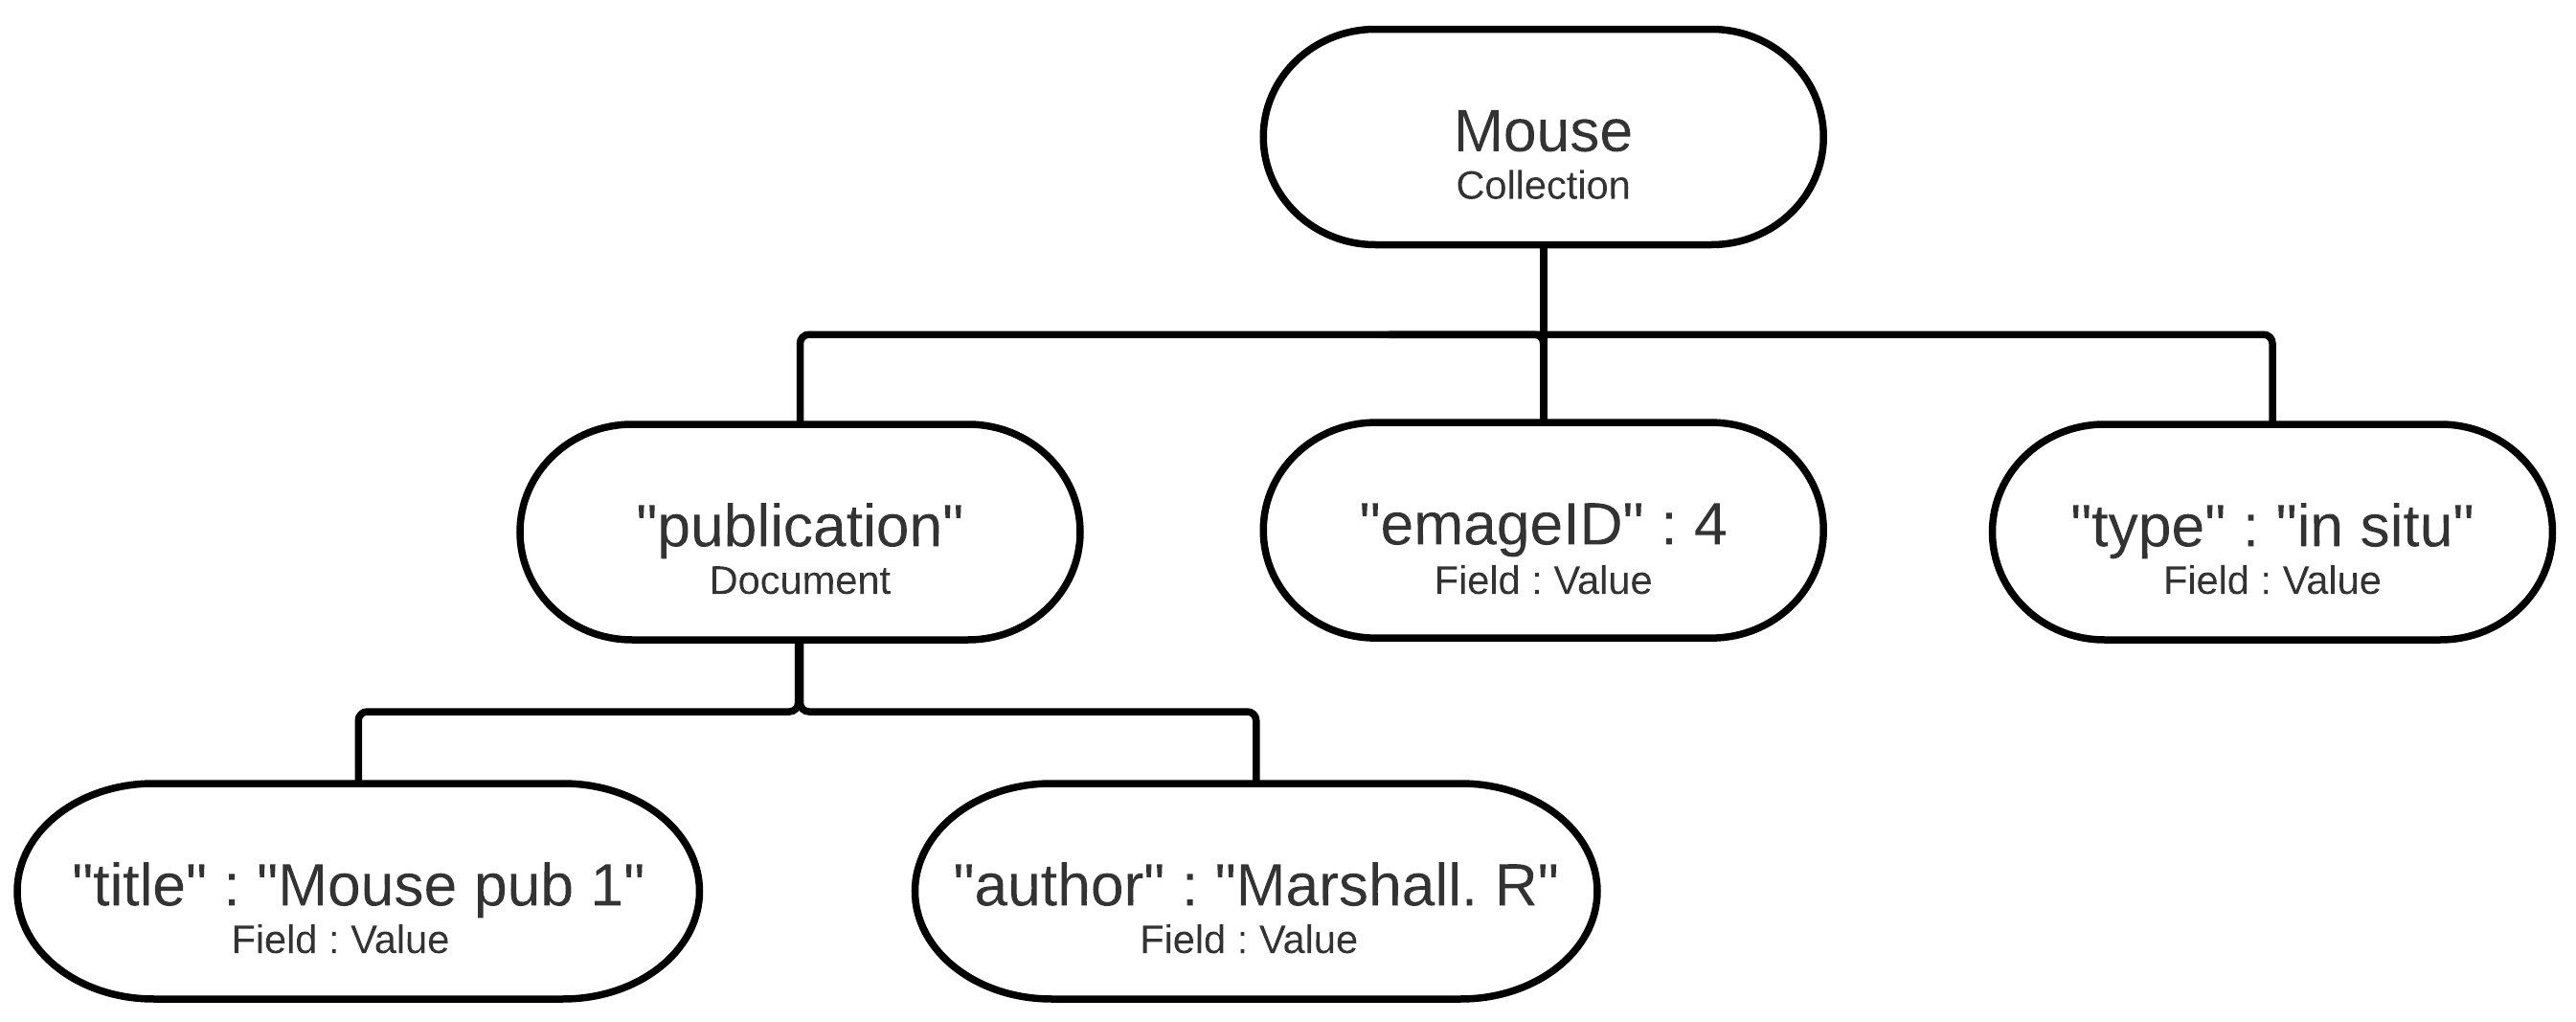
\includegraphics[width=1\linewidth]{images/embeddedex}\caption{Example of a MongoDB embedded document in a hierarchical structure.}\label{fig:embedded}\end{center}\end{figure}
\parindent 0pt
Lines 6-34 of code snippet \ref{code:mongoinsert} represent an example of data embedded in a document. Looking specifically at lines 14-20 there is a value named ``publication'' which has embedded values of ``publicationID'', ``author'' and ``title''. This allows direct querying of additional data, as opposed to messy collection joins.
\parindent 15pt
\newpage
\begin{lstlisting}[language=json,caption=Example insertion of data into a MongoDB document., label=code:mongoinsert]
db.emage.insert({
    "_id" : 5354,
    "probeID" : "Flt1 probeA",
    "source" : "emage",
    "type" : "in situ",
    "specimen" : {
        "strain" : "unspecified",
        "type" : "wholemount"
    },
    "stage" : {
        "dpc" : "9.5 dpc",
        "theilerstage" : 15
    },
    "publication" : [ 
        {
            "publicationID" : 9113979,
            "author" : "Ema M, Taya S, Yokotani N, Sogawa K, Matsuda Y, Fujii-Kuriyama Y",
            "title" : "A novel bHLH-PAS factor with close sequence similarity to hypoxia-inducible factor 1alpha regulates the VEGF expression and is potentially involved in lung and vascular development."
        }
    ],
    "textannotation" : [ 
        {
            "anatomystructure" : {
                "term" : "cardiovascular system",
                "structureID" : 16104
            },
            "strength" : "detected",
            "gene" : {
                "name" : "Flt1",
                "geneID" : "MGI:95558"
            }
        }
    ]
})
\end{lstlisting} 


\subsection{Neo4j}
To implement a Neo4j structure we use a query language namely Cypher Query Language (CQL). Cypher, is a declarative graph query language that allows for expressive and efficient querying and updating of a graph store \cite{nd}. CQL was designed to be as user friendly as possible for both programmers and operations professionals alike \cite{nd}. The structure of CQL is based upon SQL and shares many of its attributes. CQL queries are built using various clauses. For a detailed insight into CQL, see section \ref{neo}.

As Neo4j is based upon the property graph model, a database is implemented by constructing nodes and relationships. A node is made up of either a single or a number of properties. A property is a value which is named by a string. The accepted property values in Neo4j are: Numeric, String, Boolean and Collections of any other value type, for example, an array of Strings. A relationship organises the nodes by joining two nodes together on a matched value. As with nodes, relationships can have definitive value properties.

A node created in Neo4j is automatically instantiated with an ID value. Each and every node in the database has a unique numerical ID, which is incremented from the first node to the last inserted. This value can not be changed. The ID value can be used as a standalone statement or within a query clause by using the ``ID'' clause function.

Creating a Neo4j structure can be done by implementing a Cypher file; containing the indexes, nodes, constraints and relationships of the data model. The Cypher file can then be bulk loaded into the database. Alternatively a data model can be manually implemented using the Neo4j shell command prompt. Code snippet \ref{code:neocreate} is an example of how to create a structure from the command line. However, for the full EMAGE dataset instantiation, I created a Cypher file and imported the dataset simultaneously. The implementation of this is discussed in section \ref{neoload}, which also describes how to load data into Neo4j from a CSV file. Code snippet \ref{code:neocreate} illustrates the implementation of an assay, publication, indexes and constraints via the command prompt.
\newpage
\vspace*{\fill}
\begin{lstlisting}[language=SQL, caption=Example creation of an assay\, publication\, indexes and constraints in Neo4j., label=code:neocreate]
---
--- Create node indexes and constraints
---
CREATE CONSTRAINT ON (e:Assay) ASSERT e.id IS UNIQUE;
CREATE INDEX ON :Assay(emageID);
---
--- Create Assays
---
MATCH (source:Source {source : 'emage'})
MATCH (specimen:Specimen {strain : 'unspecified', type : 'wholemount'})
MATCH (stage:Stage {theilerstage : TOINT('15'), dpc : '9.5 dpc'})
CREATE (assay:Assay {emageID: TOINT('10001'), probeID : 'Epas1 probeA',
		type : 'in situ'})
CREATE (assay)-[:COMES_FROM]->(source)
CREATE (assay)-[:CLASSIFIED_AS]->(specimen)
CREATE (assay)-[:GROUPED_BY]->(stage);
---
--- Create Publications
---
MATCH (assay:Assay {emageID : TOINT('10001')})
CREATE (publication:Publication { accession: TOINT('9113979'), title : 'A novel bHLH-PAS factor with close sequence similarity to hypoxia-inducible factor 1alpha regulates the VEGF expression and is potentially involved in lung and vascular development.', author : 'Ema M, Taya S, Yokotani N, Sogawa K, Matsuda Y, Fujii-Kuriyama Y'})
CREATE (publication)-[:DESCRIBES]->(assay);
\end{lstlisting}
\vspace*{\fill}
\newpage

Creating indexes and constraints in Neo4j is a simple, one line command process for each. Lines 4 and 5 in code snippet \ref{code:neocreate} illustrate this. Imposing unique constraints on a node is more relevant when importing multiple nodes at one time by using the ``merge'' command. This is discussed in detail, in section \ref{neoload}.

As illustrated in code snippet \ref{code:neocreate}, there are 3 main stages when creating a node in my Neo4j data model. Let's take a look at the creation of the Publications node on lines 22-26. Firstly we match another node, ``Assay'', with a value which we corresponds with our publication node. In SQL terms this is essentially a join. Line 22 is saying ``Join this node I am creating, with the assay node which has an ID of 10001''. We then move on to create the publication node. To do this, we state the name of the node, then add in the field and value pairs we are looking to associate with this node, in a JSON format. Finally we create the relationship of the publication node. Line 26 represents the creation of this relationship. State the name of the parent node, define the relationship (with a string value of your choosing) then state the name of the child node. As a publication describes an assay, I have named the relationship in this case ``DESCRIBES''. The two nodes are then joined together as a result of the match we created in step 1. The ordering of this process can be rearranged. The creation of the node can come before the matching stage, however the match must come before the relationship creation. It is evident when creating a Neo4j data model, that the attributes of CQL were certainly implemented with simplicity in mind. The ease in which nodes and relationships are created is effortless.

\subsection{Apache Cassandra}\label{cassandraimplementation}
Physically creating a data model in Cassandra is similar to that of a MySQL system. They share many of the same keywords such as CREATE, WITH, SET and FROM. They also use similar key functionalities such as PRIMARY KEY. While semantically these concepts vary, the two systems are comparable syntactically.

The Cassandra data model consists of 7 tables; Assays, AssayByStage, AssayBySpecimen, Publications, StructureByGene, and TextAnnotations. Creating these tables was a simple and quick process. Despite my prior knowledge of Apache Cassandra being at a beginner level the query language CQL is instinctive to learn. This may be as a result of its similarities with SQL. Code snippet \ref{code:cassimp} illustrates the code to create each table in Cassandra. As you can see for each of the tables, the process works by giving the CREATE TABLE command, stating the table name and then stating the table columns. There are a number of different data types in Cassandra, many of which are standard such as int, double, float and boolean, with the text data type equivalent to a UTF-8 encoded string. A full description of all data types in Cassandra can be found in table \ref{tab:cassdt}.

\begin{lstlisting}[language=SQL, caption=Example of how to create tables in Cassandra., label=code:cassimp]
---
CREATE TABLE assays( emageID int, assayType text, theilerStage int, dpc text, specimenType text, specimenStrain text, probeID text, source text, PRIMARY KEY (emageID));
---
CREATE TABLE assayByStage( emageID int, theilerStage int, dpc text, probeID text, source text, PRIMARY KEY (theilerStage, emageID));
---
CREATE TABLE assayBySpecimen( emageID int, specimenType text, specimenStrain text, probeID text, source text, PRIMARY KEY (specimenType, emageID));
---
CREATE TABLE publications( publicationID text, title text, author set <text>, emageID int, PRIMARY KEY(emageID));
---
CREATE TABLE structureByGene( structureID int, structureTerm text, detected boolean, geneName text, geneID text, emageID int, PRIMARY KEY ((geneName, detected, structureID), emageID));
---
CREATE TABLE structureByStage( structureID int, structureTerm text, detected boolean, theilerStage int, dpc text, PRIMARY KEY ((theilerStage, detected), structureID));
---
CREATE TABLE textAnnotations( structureID int, structureTerm text, strength text, detected boolean, geneName text, geneID text, dpc text, theilerStage int, emageID int, PRIMARY KEY (emageid,structureID,detected);
\end{lstlisting}

Many of the keywords and concepts of Cassandra found in code snippet \ref{code:cassimp} may be familiar to the reader with a background in SQL. With the exception of the \textbf{set} data type in line 8 and the semantics of the PRIMARY KEY, everything else is for the most part the same. The set data type is a collection of one or more elements. This was imposed on the Author column of the publications table. As many of the publications contain multiple authors, using the set data type to contain each was a logical choice. The other main difference is the PRIMARY KEY operator. The primary key is split into two, a partition key and a clustering key. These values are supplied by stating PRIMARY KEY(partition key, clustering key) - lines 4 and 6 of code snippet \ref{code:cassimp}. If only one value is stipulated, then it is regarded as both the partition key and clustering key - line 2 of code snippet \ref{code:cassimp}. There can be multiple partition keys, and/or multiple clustering keys - lines 8, 10 and 12 of code snippet \ref{code:cassimp}. Each of these statements can be run on the Cassandra command-prompt and the full data model is created within seconds.

\section{Discussion}\label{schemadiscussion}
One of the major positives of MySQL is the plethora of add ons and third party tools available for modelling and general database management. Open source software such as MySQL workbench and phpMyAdmin, provide the ability to create and maintain a MySQL database, with the former providing data modelling, SQL development, and comprehensive administration tools for server configuration and user administration \cite{mysqlworkbench}. MySQL workbench also allows one to reverse engineer an ER diagram. This tool eliminates the process of manually writing the code to create tables, instantiate entities and establish table joins. All one has to do is design an ER diagram of their data model and the code is automatically generated. However, if one would prefer to manually write the script to create the data model, while potentially tedious, is not an overly time consuming process. This is the method I adopted for creating the MySQL data model.

The decision to choose this procedure was based mainly on two reasons. Firstly, I wanted to fully understand and appreciate the data modelling complexities of each database system. Secondly, I felt that using a third party tool for implementation would not result in a comprehensive evaluation of each database system. Therefore to provide an insightful perspective of the data modelling process, I implemented each system using their respective command-line interfaces. Implementing the MySQL schema was a quick procedure. I wrote the commands for each of the tables out in a text editor, verified for errors then copy and pasted into the MySQL command-line interface. My previous experience certainly helped with this stage as I was able to complete the full MySQL implementation in around twenty minutes to half an hour. 

Similar to the MySQL implementation, the creation of the Cassandra data structure was straightforward. As discussed in section \ref{designdiscussion} the most challenging part of the Cassandra modelling process was understanding what tables required creating. The procedure to develop a Cassandra data model depends on what one is looking to query and pull out of the database. Therefore the design stage effectively had already provided me with the statements to create the Cassandra model. All one has to do is run the relevant commands on the Cassandra cqlsh tool interface and the schema is implemented.

The implementation stage for the MongoDB and Neo4j data models were completed dynamically at the time of load. Therefore for comparison between the models there is not much detail to convey. These two models do not consist of a formal structure and as a result require no schema implementation. This is certainly one of the most attractive qualities of the two systems. Their flexible nature allows one to manipulate and develop a full data model with little restriction. I feel this provides a sense of control and system awareness to the developer.


